\documentclass[10pt,journal,compsoc]{IEEEtran}

% \usepackage{cite}
\usepackage[pdftex]{graphicx}
\usepackage{natbib}
% \usepackage{url}
\usepackage{hyperref}
% \usepackage{breakurl}


% \newcommand{\cm}[1]{\textbf{#1}}

\begin{document}

\title{The importance of colormaps}



\author{%
	Kristen M. Thyng
	\IEEEcompsocitemizethanks{
	\IEEEcompsocthanksitem Kristen Thyng is at Texas A\&M University in Oceanography.\protect
}}


\IEEEtitleabstractindextext{%
\begin{abstract}
Colormaps control the way data is understood when plotted because they map data values to color. When the colors used do not match the way humans perceive color, there can be a mismatch between interpretation and the data. Here I present relevant background information as well as provide suggestions as to improving colormap choices.
\end{abstract}
}


% make the title area
\maketitle


\section{Introduction}

The colors chosen to represent data in a colormap have a large influence on accurate data interpretation. One study found more mistakes in medical scan interpretation by domain experts accustomed to the rainbow-based \textbf{jet} colormap when the scan data were displayed with \textbf{jet} as compared with another colormap \citep{Spence:1999ea}. Other studies have also shown more interpretation mistakes when data is mapped with rainbow-based colormaps  \citep{borkin2011evaluation,Bryant:2014bh}. Given this, it is worth carefully considering the colormap chosen for data representation, beyond the default available or what is familiar (Fig.~\ref{fig:motivation}). The colormap information presented in this paper targets relative data (as opposed to categorical data) for which one want to understand the form and see detailed relationships in size.

Given the drawbacks of rainbow-based colormaps like \textbf{jet}, one might consider using a grayscale map for everything. While a well-made grayscale colormap can indeed be an excellent choice for data presentation, it is not the best colormap for all data. For example, grayscale would not be the best choice for representing topography and bathymetry in a single map, where introducing suggestive colors for land and water, respectively, would greatly add to the interpretability of the map. Using a distinct colormap for each variable allows for tailoring of the colormap to unique properties of each variable as well as acclimatizing viewers to the custom colormap used per variable.



\nocite{treinish1998should}
\nocite{borkin2011evaluation}
\nocite{thyng2016true}
\nocite{Spence:1999ea}



Color is represented by three dimensions, called a colorspace. All colorspaces approximate how humans see color and use different dimensions for this representation. If a colormap is created from a perceptually-uniform colorspace, it has the special property that any equal distance along the colormap is perceived by humans as approximately equal in magnitude of change (Fig.~\ref{fig:evaluation}). A consequence of not using a perceptually-uniform colormap is perceptual jumps across the colormap, which can be large. These perceptual jumps introduce fake gradients into the data representation as well as obscure detail. Another important finding from previous studies is that humans best understand the relative form of data when it is mapped by lightness rather than hue \citep{kovesi2015good}.


\nocite{kovesi2015good}



Many considerations should be taken into account when choosing the appropriate colormap for data presentation (Fig.~\ref{fig:howtochoose}):
\begin{itemize}
	\item \textbf{Use appropriate colormap type:} Colormaps for plotting relative data can be generally grouped into 3 categories. First, sequential colormaps have monotonic lightness change and should be used to represent data that increases in size (such as chlorophyll, see example in Fig.~\ref{fig:howtochoose}). Second, diverging colormaps have a monotonic increase or decrease in lightness to a point, then change to monotonically decrease or increase. The utility of a diverging colormap is in representing data values relative to a critical point (for example, sea surface height relative to mean sea level). Third, cyclic colormaps should be used to represent data that cycles around a circle, like tidal phase. They should either not vary in lightness at all and cycle through hue only, or should cycle in both lightness and hue such that there is no major perceptual break in the colormap.
	\item \textbf{Perceptual uniformity:} Use colormaps with perceptual uniformity when possible, for example, made from a perceptually-uniform colorspace like \textit{CAM02-UCS}.
	\item \textbf{Use intuition:} Use shades of green to represent changes in chlorophyll, or a colormap that goes from cool to warm colors to represent temperature.
	\item \textbf{Color blindness:} Some form of color-blindness impacts about 7\% of Northern European, 4\% of Asian, and 3\% of African-descendent men \citep{sharpe1999opsin}. Avoiding colormaps that include both red and green, which look similar with the most common form of colorblindness, would be wise to invite a wider audience to the plot.
	\item \textbf{Match colormap to data:} Choose one colormap per variable, considering the items in this list, and then stick to it for the whole presentation or paper. This way the audience will become accustomed to the meaning of the colors and be able to quickly determine meaning from plots without extensive study of the colorbar and legend.
	\item \textbf{Magnitude vs. range:} Some sequential variables have a clear meaning of magnitude, like turbidity or turbulence, and others measure a metric, like temperature. For the former, consider a colormap with shades of one color, where increasing shades represent increasing size of the variable. For the latter, consider a colormap that traverses several colors so that there is always a color representing the range of data values instead of white, which could connote the absense of the variable.
\end{itemize}




A wide variety of reasonable, available colormaps are presented in Fig.~\ref{fig:allmaps} \citep{hunter2007matplotlib,light2004end,brewer,crameri2018geodynamic,mycarta}. Colormaps are plotted by the lightness as calculated in perceptually-uniform colorspace \textit{CAM02-UCS} in order to demonstrate this important property for making a colormap choice.

% colormaps



\section{Conclusion}

Colormaps have fundamental control over interpretation of data, and thus should be given careful attention. Human perception of color as well as basic design advice should guide selections.

The notebook used to create the base figures in this paper can be found at \url{https://github.com/kthyng/cise-colormaps}.


\section{Acknowledgments}

Plots were created using the following Python packages: Matplotlib, Jupyter, numpy, xarray, pandas, cartopy, and colorspacious along with the colormaps packages cmocean, colorcet, and palettable.



\bibliographystyle{IEEEtran}
\bibliography{./refs}

\bigskip

\textbf{Kristen Thyng} is an assistant research professor of oceanography at Texas A\&M University. Her research interests include coastal physics, numerical modeling, visualization, and data science. She received a Ph.D. in mechanical engineering from the University of Washington, USA. Contact her at kthyng@tamu.edu.

\begin{figure*}
	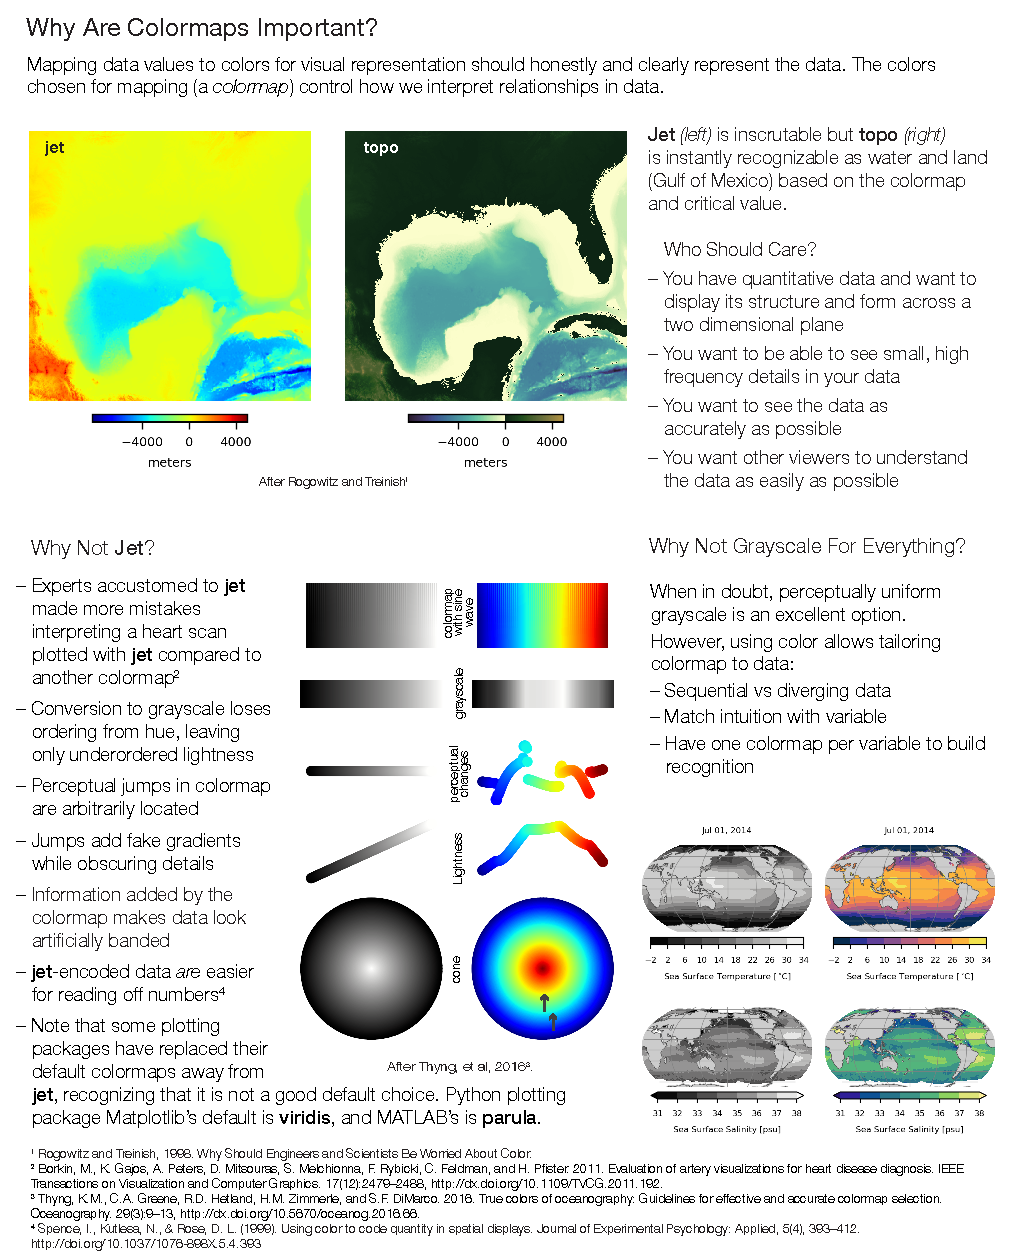
\includegraphics[width=\textwidth]{figures/motivation.pdf}
	\caption{Figure available under CC-BY (10.6084/m9.figshare.12594737).}
	\label{fig:motivation}
\end{figure*}

\begin{figure*}
	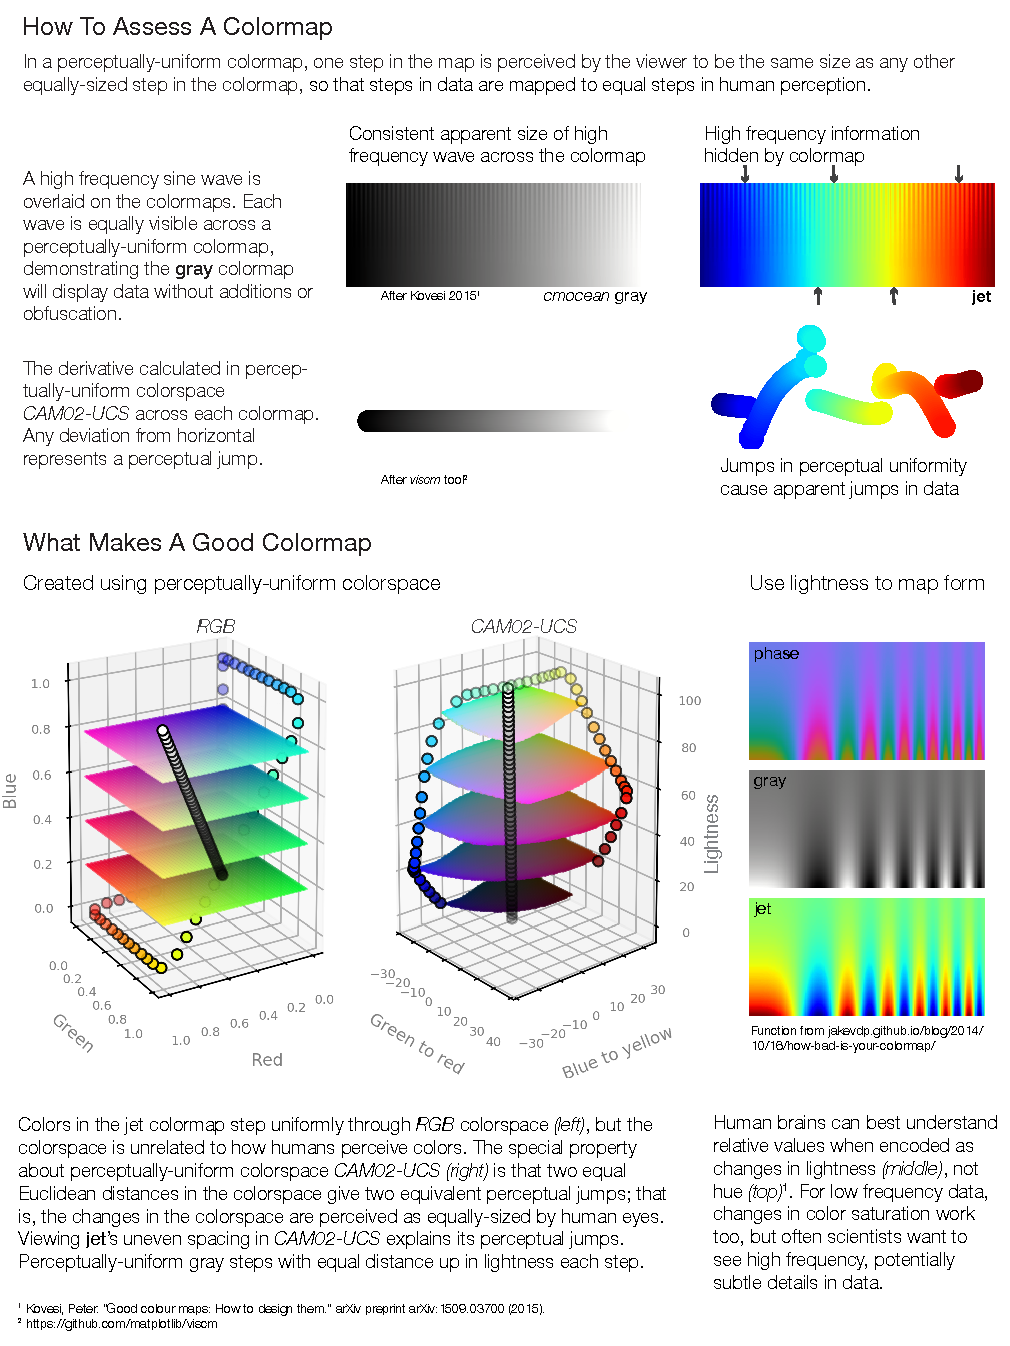
\includegraphics[width=\textwidth]{figures/evaluation.pdf}
	\caption{Figure available under CC-BY (10.6084/m9.figshare.12597170).}
	\label{fig:evaluation}
\end{figure*}

\begin{figure*}
	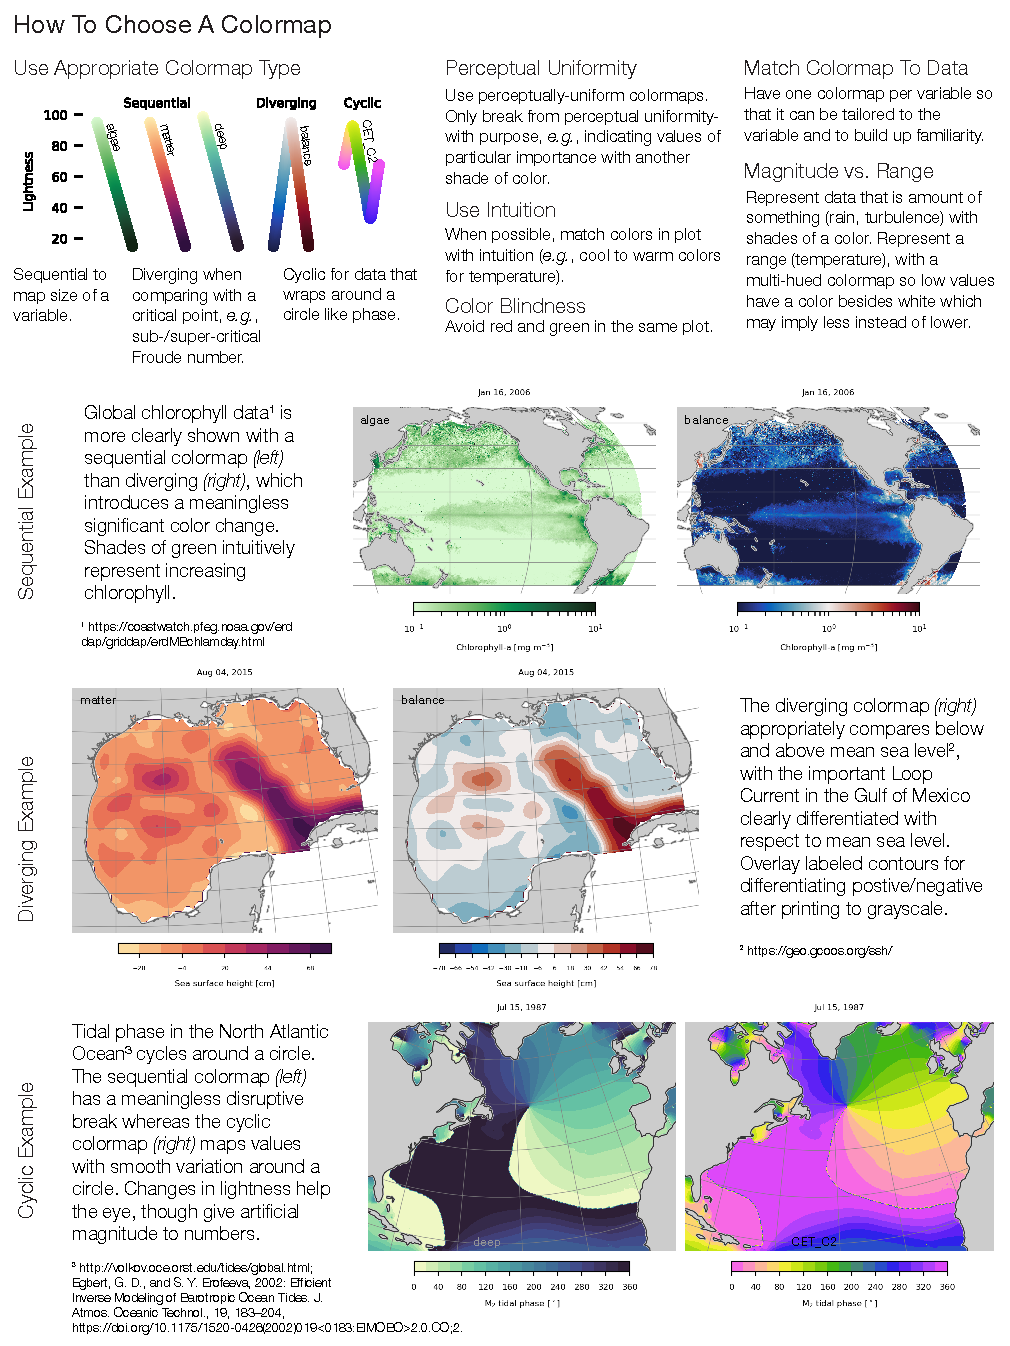
\includegraphics[width=\textwidth]{figures/howtochoose.pdf}
	\caption{Figure available under CC-BY (10.6084/m9.figshare.12597197).}
	\label{fig:howtochoose}
\end{figure*}

\begin{figure*}
	\includegraphics[width=\textwidth]{figures/allmaps.pdf}
	\caption{Figure available under CC-BY (10.6084/m9.figshare.12597206).}
	\label{fig:allmaps}
\end{figure*}


\end{document}
